\documentclass[11pt]{article}
\usepackage[utf8]{inputenc}
\usepackage[T1]{fontenc}
\usepackage[french]{babel}
\usepackage{amsmath}
\usepackage[bookmarks={true},bookmarksopen={true}]{hyperref}
\usepackage{graphicx}
\usepackage[a4paper]{geometry}
\usepackage{listings}
\usepackage{hyperref}
\usepackage{amssymb}
\usepackage{amsmath,amsfonts}
	\lstset{frame=tb,
		language=Java,
 		aboveskip=3mm,
  		belowskip=3mm,
  		showstringspaces=false,
  		columns=flexible,
  		basicstyle={\small\ttfamily},
  		numbers=none,
 		numberstyle=\tiny\color{gray},
  		keywordstyle=\color{blue},
  		commentstyle=\color{dkgreen},
  		stringstyle=\color{mauve},
  		breaklines=true,
  		breakatwhitespace=true
  		tabsize=3
	}
\pagestyle{plain}
\setlength{\parindent}{5mm}
\usepackage{amsmath}
\usepackage{color}
\definecolor{dkgreen}{rgb}{0,0.6,0}
\definecolor{gray}{rgb}{0.5,0.5,0.5}
\definecolor{mauve}{rgb}{0.58,0,0.82}



\title{\textbf{Projet LSINF1121 -  Algorithmique et structures de données\\ - \\ Rapport intermédiaire Mission 6} \\ {\large Groupe 26}}
\author{Laurian \bsc{Detiffe} \\(6380-12-00)\and Sundeep \bsc{Dhillon} \\(6401-11-00)\and Alexis \bsc{Macq} \\ (5910-12-00) \and Xavier \bsc{Pérignon} \\ (8025-11-00)\and Thibaut \bsc{Piquard}\\(4634-13-00)\and Thomas \bsc{Wyckmans} \\ (3601-12-00)}
\date{date}
\date{\vspace*{25mm}

\includegraphics[scale=0.75]{logo.jpg}\\
		\vspace*{30mm}
		\begin{center}
		Année académique 2015-2016 \\	
		\end{center}}

\begin{document}
\thispagestyle{empty}

\maketitle
\thispagestyle{empty}
%\tableofcontents
%\setcounter{tocdepth}{3}
%\setcounter{page}{1}
%\newpage

\section*{Questions et réponses}
\begin{enumerate}

\item \textit{Quelles sont structures de données alternatives pour représenter un graphe G
non dirigé comportant n noeuds (vertex) et m arcs (edges). Quelles sont les
complexités des opérations élémentaires \texttt{Iterable <Integer> adj(int
v) et addEdge(int v, int w)}.} (Sundeep) \medskip

Il existe trois structures de données permettant de représenter un graphe G non dirigé comportant $n$ noeuds et $m$ arcs, à savoir:
\begin{enumerate}
\item \textbf{Une matrice d'adjacence}: il s'agit d'un tableau de booléens dont les lignes et les colonnes correspondent aux noeuds du graphe G non dirigé.
\item \textbf{Un tableau d'arcs}: c'est un tableau composé de deux variables correspondant aux deux noeuds qui sont liés par une certain arc.
\item \textbf{Un tableau de liste d'adjacences} : c'est un tableau dont chacune des entrées représente un certain noeud auquel est affecté une liste d'adjacences.
\end{enumerate}
Ci-dessous, vous trouverez un tableau comprenant les complexités des opérations élémentaires des différentes structures de données énoncées plus haut:
\begin{table}[h!]
\begin{center}
\begin{tabular}{ |c|c|c|c| } 
\hline
 \texttt{Structure de données} & \texttt{adj(int v)} & \texttt{addEdge(int v, int w)} \\
  
  \hline Matrice d'adjacence & $O(V)$ & $O(1)$ \\ 
  \hline Tableau d'arcs & $O(E)$ & $O(1)$ \\ 
  \hline Tableau de liste d'adjacences & $O(degré(v))$ & $O(1)$\\
  \hline
\end{tabular}
\end{center}
\end{table}


\item \textit{Un graphe est biparti si ses noeuds peuvent être divisés en deux ensembles disjoints de sorte qu’il n’existe pas d’arc entre deux noeuds du même ensemble.
Proposez une méthode pour tester si un graphe est biparti et si oui qui trouverait
une telle partition. Quelle est la complexité de votre algorithme ? Hint : utilisez
un DFS.}(Sundeep) \medskip

La complexité de l'algorithme ci-dessous est de l'ordre de $O(V+E)$.\\
\begin{lstlisting}
public class Bipartite{
    
    private boolean[] markedYes; // markedYes[v] = true si v a ete visite en DFS
    private boolean[] markedNo; // markedNo[v]nous fournit les sommets d'un cote du graphe bipartite
    private boolean isBipartite; // est-ce que le graphe G est bipartite?
    private int count;
    
    public Bipartite(Graph G, int s){
        this.markedAsYes = new boolean[G.V()];
        this.markedAsNo = new boolean[G.V()];
        this.isBipartite = true;
        this.count = 0;        
        dfsYes(G, s);
    }
    
    private void dfsYes(Graph G, int v){
        markedAsYes[v] = true;
        count++;
        for (int w : G.adj(v)){
            if (markedYes[w]){ // si v-w cree un certain cycle, il faut le trouver
                isBipartite = false;
            }
                
            if (!markedNo[w]) dfsNo(G, w); // on a trouve un sommet d'un cote du graphe bipartite, on reitere
        }
    }

    private void dfsNo(Graph G, int v){
        markedNo[v] = true;
        count++;
        for (int w : G.adj(v)){
            if (markedNo[w]){
                isBipartite = false;
                return;
            }
            
            if (!markedYes[w]) dfsYes(G, w);
        }
    }
    
    public boolean isBipartite(){ // renvoie true si le graphe est bipartite et false dans le cas contraire
        return isBipartite;
    }
    
    public int count(){
        return count;
    }
    
    public boolean[] markedYes(){
        return markedYes;
    }
    
    public boolean[] markedNo(){
        return markedNo;
    }
}
\end{lstlisting}

\item \textit{Prouvez que tout graphe connecté a un noeud dont le retrait (y comprit des arcs incidents) ne déconnecterait pas le graphe. Ecrivez une méthode qui trouve un
tel noeud. Hint : utilisez un DFS et le marquage des noeuds.} (Sundeep) \medskip

Dans le cas où nous avons un graphe connexe non cyclique, nous n'avons besoin d'aucune preuve car on remarque facilement qu'un noeud positionné à l'extrémité du graphe peut être retiré sans enlever la propriété connexe de ce dernier.\\
Par contre, supposons que nous faisons face à un graphe G connexe cyclique, composé des noeuds $v_1, v_2, ..., v_n$ formant un cycle tel que $v_1 \Rightarrow v_2$ ($=$ $v_1$ connecté à $v_2$), $v_2 \Rightarrow v_3$, ... , $v_n \Rightarrow v_1$. Le fait d'enlever un noeud du cycle transforme notre graphe G en graphe connexe non cyclique, qui est donc toujours un graphe connexe. On peut donc toujours enlever un des noeuds du cycle d'un graphe connexe cyclique sans perdre la propriété de connexité. L'algorithme est applicable dans le cas ou un noeud du cycle est relié à un sous-graphe cyclique. De plus, si un des noeuds du cycle est relié à un sous arbre non cyclique, le raisonnement développé au dessus est d'application. 
\subsection*{Méthode: trouver un noeud déconnectable}
Une des méthodes possible serait d'utiliser une variante de l'algorithme de \textit{depth-first search} (DFS): On parcours chaque noeud du graphe un à un. Pour chacun, on vérifie si le noeud adjacent à chacune de ses arrêtes est marqué. Si oui, le noeud et ses arrêtes peuvent être retirés sans que le graphe ne perde son caractère connexe. Si non, on marque le noeud et on réitère avec un des noeuds adjacents non marqué.






\item La solution est d'utiliser un Breadth-first search (BFS). En fesant celà, on trouve les noeuds adjacents au départ.Si ceux-ci ont déjà étés visités, on les ignore. Autrement, on l'ajoute aux éléments du tableau qui renverra le chemin le plus cour.  On réitère cette opération jusqu'à atteindre la sortie. On renvoie ensuite le tableau obtenu qui nous donnera le chemin désiré. 
Notre complexité sera de O(n*p) pour une matrice d'ajacence et celà peut diférer selon l'implémentation.

\begin{lstlisting}

Private void bfs(Graph G, int debut,int finish)
{
	Queue<Integer> q = new Queue<Integer>();
	IsAlreadyVisited[debut] = true;
	q.enqueue(debut)
	while(!q.isEmpty())
	{
	int v = q.dequeue();
	if ( v == finish)
		{
		break;
		}
	for (int w : G.adjacent(v))
		if(! IsAlreadyVisited[w])
		{
			path[w] = v ;
			 IsAlreadyVisited[w] = true;
			queue.enqueue(w);
		}
	}
}
\end{lstlisting} 

\item On utilise un Depth-first search(DFS) qui vérifie à chaque fois dans le cas ou le noeud trouvé a déjà été visité si c'est un noeud déjà parcouru dans ce chemin du DFS. Dans ce cas, il y a cycle.

\begin{lstlisting}
Public boolean hasCycle(Graph G,  int v,  int u,hasCycle)
{
	 IsAlreadyVisited[v];
	for ( int w : G.adjacent(v))
		{
		if(! IsAlreadyVisited[w])
		{
			dfs(G,w,v,hasCycle);
		}
		else if (w!=u) hasCycle = true;
		}
	return hasCycle;
}
\end{lstlisting} 

\item 
\begin{lstlisting}
Public void Topologic(Graph G,int n)
{
	Int[]d = new Int[n]
	Queue<Integer> q = new Queue<Integer>();
	int k;
	for (int i=0; i++;i <= n)
	{
		d[i]=i.degre()
		if(d[i]==0)
		{
			q.add(i)
		}
	}
	while(!q.isEmpty())
	{
		k=q.remove()
		d[k]=d[k]-1;
		for(int i : G.adjacent(k))
		{
			d[i]=d[i]-1;
			if(d[i]==0)
			{
				q.add(i)
			}
		}
	}
}

\end{lstlisting} 

\item Afin de compléter le MST partiel et retrouver un MST complet dans le graphe G, je vais appliquer l’algorithme de Kruskal. Cet algorithme est simple, il récupère tous les Lien (Edge) triés de manière croissante (plus petit poids au plus grand) et va ajouter au fur et à mesure tous ceux qui ne forme pas de cycle :
\\
\begin{lstlisting}
Public static void RecoverMST(EdgeWeightedGraph G, Queue<Edge>, UF uf)
{
	MinPQ<Edge> pq = new MinPQ<Edge>(G.edges());
	while (!pq.isEmpty() && mst.size() < G.V()-1)
	{
		Edge e = pq.delMin();   		 //Get min weight edge on pq
		int v = e.either(), w = e.other(v); 	//and its vertices.
		If (uf.connected(v,w))  {continue;}	//ignore ineligible edges.
		uf.union(v,w); 				//merge components 
		mst.enqueue(e);				//Add edge to mst
	}
}
\end{lstlisting} 

\url{http://algs4.cs.princeton.edu/43mst/KruskalMST.java.html}
\\
\\
Cet algorithme se base sur une règle fondamentale du MST, il nepeut y avoir de cycle à l’intérieur d’un MST. Grâce à « union-find », on peut savoir si deux somments sont déjà connectés ou non, et s’il faut donc traiter cet Edge (l’ajouter au MST).
\\
Il est aussi possible de régénérer l’union-find depuis le MST existant, simplement en parcourant celui-ci et en liant chacun des différents sommets dans chacune des liants de ce MST partiel.
La complexité temporelle de cette méthode est de O(Elog(E)).\\

\item On peut élargir ce problème à un problème de MST plus vaste, c’est-à-dire : comment mettre à jour votre MST après un Edge quelconque  ait été mis à jour dans votre Graphe ? \\
Il y a plusieurs cas possible :
\begin{enumerate}
	
	\item L’edge mis à jour est dans votre MST et sa valeur décroît : il n’y a strictement rien à faire.
	\item L’edge mis à jour n’appartient pas au MST et sa valeur décroît : il faut ajouter l’Edge dans le MST, ce qui créera un 		cycle au sein du MST. Il suffit ensuite de parcourir le MST depuis un des deux Vertice de cet Edge (via BFS ou DFS) et 			retirer dans ce cycle l’Edge au poids le plus haut (Complexité O(N)).
	\item L’Edge mis à jour est dans votre MST et sa valeur croît : il faut retirer  l’Edge de cet MST, ce qui créera deux éléments connectés qui doivent être raccordés. On peut facilement calculer ces deux composants via DFS ou BFS (Complexité O	(N)), il faut ensuite parcourir les Edge restants par ordre croissant et ajouter le premier Edge qui relie les deux éléments connectés.
	\item L’Edge mis à jour ne fait pas partie du MST et sa valeur croît : Le MST actuel est toujours un MST.
	
	\end{enumerate}
<<<<<<< HEAD
Maintenant, ces différents cas ne couvrent pas spécifiquement notre problème tel que je le comprends, c’est-à-dire, inclure quoi qu’il arrive l4Edge e même si celui-ci ne devrait pas se trouver dans le MST. Pour arriver à résoudre ce problème, il suffit de tweaker un petit peu le cas 2. Au moment du retrait du poids le plus haut, si celui-ci est l’Edge e, alors on retirera le second plus haut.
=======

Maintenant, ces diffétents cas ne couvrent pas spécifiquement notre probléme tel que je le comprends, c’est-à-dire, inclure quoi qu’il arrive l4Edge e même si celui-ci ne devrait pas se trouver dans le MST. Pour arriver à résoudre ce problème, il suffit de tweaker un petit peu le cas 2. Au moment du retrait du poids le plus haut, si celui-ci est l’Edge e, alors on retirera le second plus haut.\\
>>>>>>> origin/master


\item Oui, en utilisant une priority queue qui contiendrait les noeuds candidats à la prochaine
relaxation de la manière suivante :\\
\par 1 - On ajoute le noeud source s à un arbre et ses noeuds adjacents à la priority 
queue avec leur distance à s comme clef.\\
\par 2 - On retire de la priority queue le noeud n de clef minimale, on le rajoutte
 à l'arbre (= on le relaxe) et on ajoute ses voisins à la queue de priorité avec comme
 clefs leur distances à n + la distance de n à s comme étant leurs distance à s si 
 celle-ci est plus petite que la distance à s actuelle ou si celle-ci est la première
 distance à s ajoutée pour le noeud en cours de traitement.\\
\par 3 - On répète l'étape 2 jusqu'à ce que chaque noeud ait été ajouté et retiré une fois
 de la priority queue.\\
L'arbre ainsi formé contient les plus courts chemins de s à tout noeud v de V.\\
\par L'algo de Dijkstra a une complexité spatiale proportionnelle à |V| et une complexité
 temporelle proportionnelle à |E|log(|V|) dans le pire des cas pour calculer tous les 
 plus courts chemins des noeuds de V à une source appartenant à V.
\par Démonstration :\\
Le bottleneck dans cet algorithme est le nombre de comparaisons entre clefs des noeuds
 dans les méthodes insert() et delMin() de la priority queue. Le nombre de noeuds dans 
 la priority queue est au plus |V| ce qui nous donne la complexité spatiale.\\
 Dans le pire des cas, le coût d'une insertion est proportionnel à log(|V|) et le coût
 d'une suppression est proportionnel à 2log(|V|). Puisqu'on a au plus |V| noeuds inséré
 et |V| noeuds supprimés, la complexité temporelle est |E|log(|V|).\\

(Alexis)\\

\item Soit le graphe suivant :\\

\begin{figure}[h!]
    \center
    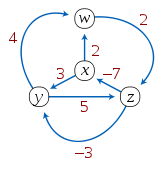
\includegraphics[width=5cm]{graph.png}
    \caption{Graphe contenant un cycle de longueur impaire (w-z-x)}
\end{figure}
<<<<<<< HEAD
=======

>>>>>>> origin/master
En empruntant le cycle w-z-x une infinité de fois, on sait montrer que 
la distance minimale entre y et w est $ -\infty $ 
or en appliquant l'algorithme de Dijkstra, 
on ne peut relaxé qu'une fois chaque noeud ce qui implique qu'on ne peut parcourir
le cycle w-z-x de longueur négative qu'une et une seule fois et l'algorithme 
de Dijkstra ne pourra donc pas nous permettre d'obtenir la solution optimale,
 à savoir $ -\infty $. Il gardera toutefois la même complexité malgré la présence de poids négatifs puisqu'en appliquant 
 l'algorithme de Dijkstra, on ne peut relaxé qu'une seule fois chaque noeud.\\

(Alexis)\\

\item \textit{Soit $G$ un graphe avec des poids potentiellement négatif mais il n’y a pas de
cycle négatif. Je cherche le chemin le plus court entre un noeud $u$ et un noeuds $v$.
J’ai à ma disposition une implémentation de Dijkstra qui ne permet pas de gérer
les poids négatifs. Il me suffit dès lors d’augmenter tous les poids d’une même
quantité correspondant a la valeur absolue du plus petit poids et d’appliquer
Dijkstra sur ce graphe. Cette méthode est-elle valable ? Si non, montrez un contre
exemple.} (Xavier)\\

Non, c'est méthode n'est pas valable. Par exemple, considérons le graphe où il existe deux chemins de A vers B, l'un traversant un seul arc de longueur 2, et l'autre traversant des arcs de longueur 1, 1 et -2. Le deuxième chemin est plus court, mais si on augmente de 2 tous les poids des arcs (valeur absolue du plus petit poids), le premier chemin a maintenant une longueur de 4, et le second a une longueur de 6, inversant le chemin le plus courts.
\begin{center}
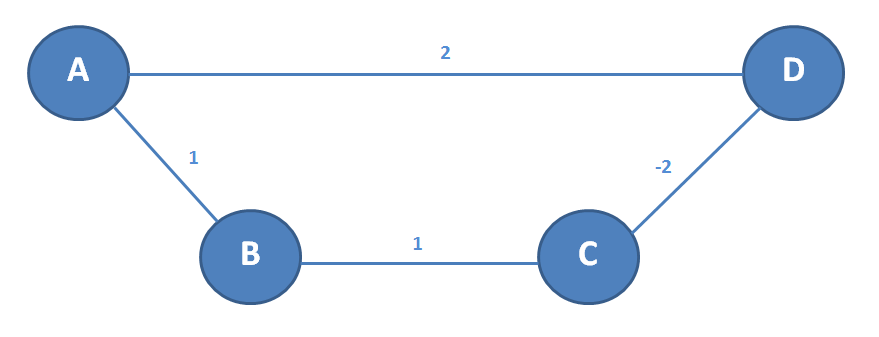
\includegraphics[scale=0.5]{dijk.PNG} 
\end{center}
Cette méthode ne fonctionnera que si tous les chemins possibles entre les deux noeuds utilisent le même nombre d'arcs.\\

\item \textit{Soit $G$ un graphe avec des poids positifs. Je cherche le chemin le plus long entre
un noeud $u$ et un noeuds $v$. J’ai à ma disposition l’implémentation de Bellman-
Ford (qui supporte les poids négatifs). Il me suffit dès lors de calculer le plus
court chemin sur le même graphe avec l’opposé des poids. Est-ce que cette méthode
est valable ? Si non pouvez-vous proposer une méthode pour le calcul de
plus long chemin ? Votre méthode s’applique-t-elle à tous les graphes ? Si non
quels-types particuliers de graphes peut-elle gérer ?} (Xavier)\\

Cette méthode est valable pour certains graphes. Le principe le plus important pour l'utilisation de cette méthode est qu'il n'y ait pas de cycle dans le graphe, dans laquelle les arcs ont une somme négative. Dans ce cas, une boucle infinie serait générée et aucun plus long chemin ne serait trouvé.

\end{enumerate}
\end{document}
